\chapter{\acrshort{api} - \acrlong{api}}

\section{Autenticazione}
\label{chap:api}

Il sistema gestisce l'autenticazione degli utenti e le loro autorizzazioni utilizzando \gls{jwt}. Il \gls{backend} dell'applicazione espone delle \acrshort{rest} \acrshort{api} \textit{state-less}, ovvero che non mantengono nessuna sessione sugli utenti autenticati, ma che si aspettano piuttosto di ricevere in ogni chiamata un \textit{token} che contiene l'identificazione del chiamante. \\

\noindent
Nella fase di login, quando un utente effettua l'accesso al proprio account, viene invocato il metodo \textit{login} di \textit{AuthController}, che ritorna ritorna un oggetto contenente:
\begin{itemize}[itemsep=0pt]
	\item l'utente che ha effettuato l'accesso
	\item un flag booleano che indica se l'utente è nuovo o meno
	\item un \textit{token} \acrshort{jwt}, il cui contenuto è l'utente che ha eseguito il login, firmato con la chiave privata del server
\end{itemize}

\noindent 
Il \textit{token} generato dovrà essere incluso in ogni chiamata autenticata che l'applicazione \gls{frontend} desidera effettuare.

\subsection{\Gls{backend}}
\label{chap:auth-backend}
\expressjs~fornisce la possibilità di utilizzare delle funzioni, chiamate \textit{middleware}, prima che un metodo venga eseguito. Esse vengono eseguite in serie, permettendo di definire in funzioni atomiche controlli di validazione sulla chiamata in cui vengono innestate.

Tutti i \textit{\nameref{server:controllers}} dell'applicazione \nodejs~derivano da un \textit{BaseController} che espone un metodo, \textit{useAuth}.

\begin{figure}[H] 
	\centering    
	\lstinputlisting{Chapter4/base-controller.ts}
	\caption[Metodo \textit{useAuth} di \textit{AuthContoller}]{Metodo \textit{useAuth} di \textit{AuthContoller}}
	\label{fig:server-base-controller}
\end{figure}

\noindent
Questo metodo registra un nuovo \textit{middleware} che ha due funzioni:
\begin{enumerate}
	\item verifica che la chiamata corrente contenga nell'\textit{header} \acrshort{http} un \textit{token} valido e non scaduto
	\item aggiunge al parametro \textit{req.body} una nuova proprietà che contiene il risultato della decodifica del token \acrshort{jwt} (ovvero un oggetto \textit{User}, con i relativi ruoli)
\end{enumerate}
Il \textit{middleware} di autenticazione viene eseguito in tutte le chiamate che vengono registrate dopo di lui. Il metodo \textit{useAuth} deve venire infatti chiamato prima di tutti i metodi che utilizzano l'autenticazione e dopo di tutti quelli che non la utilizzano. Per esempio, in figura \ref{fig:server-bootstrap} il metodo \textit{useAuth} è chiamato all'inizio, il che significa che tutti i metodi di \textit{InternshipController} sono protetti da autenticazione.

\begin{figure}[H] 
	\centering    
	\lstinputlisting{Chapter4/auth-middleware.ts}
	\caption[\textit{AuthMiddleware} di \textit{AuthContoller}]{\textit{AuthMiddleware} di \textit{AuthContoller}}
	\label{fig:server-auth-middleware}
\end{figure}

\subsubsection{\textit{Authentication scopes}}
\label{server:scopes}
Tutti i metodi registrati dopo l'utilizzo di \textit{useAuth} vengono quindi eseguiti se e soltanto se la chiamata contiene un \textit{token} valido. Durante la loro esecuzione esisterà dunque una proprietà che contiene l'oggetto \textit{User} che ha effettuato la chiamata, e sarà quindi possibile permettere di arrestarne l'esecuzione se l'utente corrente non dovesse disporre del ruolo necessario per eseguirla.

Con questa filosofia ho creato dei \textit{middleware} di autorizzazione predefiniti, chiamati \textit{scopes}, che permettono di autorizzare solo una tipologia di utenti. Gli \textit{scopes} inseriti all'interno dell'applicazione sono:
\begin{itemize}[itemsep=0pt]
	\item \textit{adminScope}: permette l'esecuzione se l'utente corrente contiene almeno il ruolo \textit{Admin}
	\item \textit{companyScope}: permette l'esecuzione se l'utente corrente contiene almeno il ruolo \textit{Company}
	\item \textit{studentScope}: permette l'esecuzione se l'utente corrente contiene almeno il ruolo \textit{Student}
	\item \textit{professorScope}: permette l'esecuzione se l'utente corrente contiene almeno il ruolo \textit{Professor}
	\item \textit{ownCompanyScope}: permette l'esecuzione se l'utente corrente è un amministratore dell'azienda su cui sta eseguendo l'operazione
	\item \textit{ownInternshipScope}: permette l'esecuzione se l'utente corrente è proprietario del tirocinio su cui sta eseguendo l'operazione
	\item \textit{ownInternshipProposalScope}: permette l'esecuzione se l'utente corrente è un un soggetto (azienda, professore o studente) della proposta di tirocinio su cui sta eseguendo l'operazione
\end{itemize}
Gli \textit{scopes} si possono anche combinare insieme in serie per ottenere autorizzazioni più articolate.

\subsection{\Gls{frontend}}
\label{chap:client:authentication}
\subsubsection{Autenticazione nei \textit{\hyperref[client:services]{Services}}}
L'applicazione \angular~deve ovviamente preoccuparsi di inserire nell'\textit{header} (\acrshort{http}) di tutte le chiamata autenticate il \textit{token} ricevuto al login, dal momento che il server non mantiene nessuna sessione per gli utenti autenticati. Questa logica è inserita all'interno del \textit{BaseService} da cui tutti i \textit{\hyperref[client:services]{Services}} derivano: questa classe espone dei metodi nominati con il \textit{verb} \acrshort{http} che si intende utilizzare. Ha una dipendenza nei confronti di \textit{AuthService} --- che non deriva da \textit{BaseService}, ma espone i metodi di login e registrazione --- per il recupero del \textit{token} corrente.

\begin{figure}[H] 
	\centering    
	\lstinputlisting{Chapter4/base-service.ts}
	\caption[Esempio di metodo esposto da \textit{BaseService}]{Esempio di metodo esposto da \textit{BaseService}}
	\label{fig:client-auth-base-service}
\end{figure}

\subsubsection{Autenticazione nei \textit{\hyperref[client:modules]{NgModules}}}

Il modulo che contiene la porzione di applicazione visibile dopo l'autenticazione, \textit{\nameref{client:auth-module}}, per essere caricato con il \textit{lazy-loading} richiede solamente che l'utente sia autenticato e disponga di un token valido. A questo livello non è ancora necessaria l'autorizzazione basata sui ruoli in quanto questo modulo e i suoi sotto moduli comprendono pagine condivise raggiungibili da utenti con ruoli differenti.

L'autorizzazione basata sui ruoli viene infatti applicata a livello di pagina: ad ogni componente registrato nel router di \angular, sono associati uno o più ruoli necessari per accedervi. Nel caso in cui il \textit{token} non contenga un \textit{claim} valido, l'utente viene reindirizzato in una pagina di errore 404.

\section{Endpoints}

Tutti i \hyperref[server:controllers]{\textit{controllers}} dell'applicazione \expressjs~ritornano i risultati delle chiamate all'interno di un oggetto standard chiamato \textit{ApiResponseDto<T>} che contiene oltre al risultato dell'operazione delle altre informazioni, come lo stato \acrshort{http} ed eventuali errori. Tutti i \textit{controllers} sono esposti sotto al path convenzionale "/api".

\subsection{BaseController}
\label{server:base-controller}
Il \textit{BaseController} espone di default i metodi \acrshort{crud} dell'entità parametrica del \textit{controller} che lo estende, in modo tale da non dover riscrivere codice duplicato. I metodi che rende disponibile ai figli sono esposti nella tabella \ref{table:endpoints}.

\begin{table}[h]
    \ttfamily
    \caption{Endpoint \hyperref[server:base-controller]{\textit{BaseController}}}
    \centering
    \label{table:endpoints}
    \begin{tabular}{l c c c c}    
    URL  & Metodo & Parametri  & Risposta & Scope \\ 
	    \midrule
	    /<controllerName> & GET &  & Array<T>   \\
	    /<controllerName>/:id & GET & string & Array<T>   \\
	    /<controllerName> & POST & T & T  \\
	    /<controllerName> & PUT & T & T  \\
	    /<controllerName>/:id & DELETE & string & boolean  & adminScope \\
	    \bottomrule
    \end{tabular}
\end{table}

\noindent
Nel caso un \textit{controller} derivato non intenda esporre alcuni di questi metodi, è sufficiente in fase di registrazione del \textit{controller} stesso passare delle opzioni al metodo \textit{useCrud(options: CrudOptions)}, specificando i metodi disabilitati oppure \textit{scopes} aggiuntivi.

Il \textit{BaseController} ha una dipendenza dall'applicazione di \expressjs, in quanto deve averne accesso per registrare nuovi metodi nel suo \textit{router}.

\subsection{InternshipsController}
Questo \textit{controller} gestisce le operazioni sui tirocini. Il suo path è "/internships".
\subsubsection{Dipendenze}
\begin{itemize}[itemsep=0pt]
	\item \textit{internshipsRepository: InternshipsRepository}
\end{itemize}
\subsubsection{Endpoint}
\label{server:internship-controller}
\begin{table}[H]
	\ttfamily
	\caption{Endpoint \hyperref[server:internship-controller]{\textit{InternshipController}}}
	\centering
	\label{table:api:internship-controller}
	\begin{tabular}{l c c c c}    
		URL  & Metodo & Scope \\ 
		\midrule
		/getByCompanyOwnerId/:ownerId & GET    \\
		/getApproved & GET   \\
		/getNotApproved & GET   \\
		/status & PUT & professorScope \\
		/status/force & PUT & adminScope \\
		/status/:status & GET \\
		\bottomrule
	\end{tabular}
\end{table}

Gli ultimi tre metodi in tabella sono utilizzati per aggiornare lo stato di un tirocinio:
\begin{itemize}
	\item PUT "/status": permette di aggiornare lo stato di un tirocinio (es. da "Non approvato" ad "Approvato"). Dal momento che gli stati dei tirocini seguono una macchina a stati ben definita, questo metodo verifica che il nuovo stato sia raggiungibile dallo stato corrente e che l'utente che ha effettuato la richiesta abbia il permesso di effettuare questa transizione. La definizione della macchina a stati è riportata in figura \ref{fig:internship-state-machine}.
	 \begin{figure}[H] 
		\centering    
		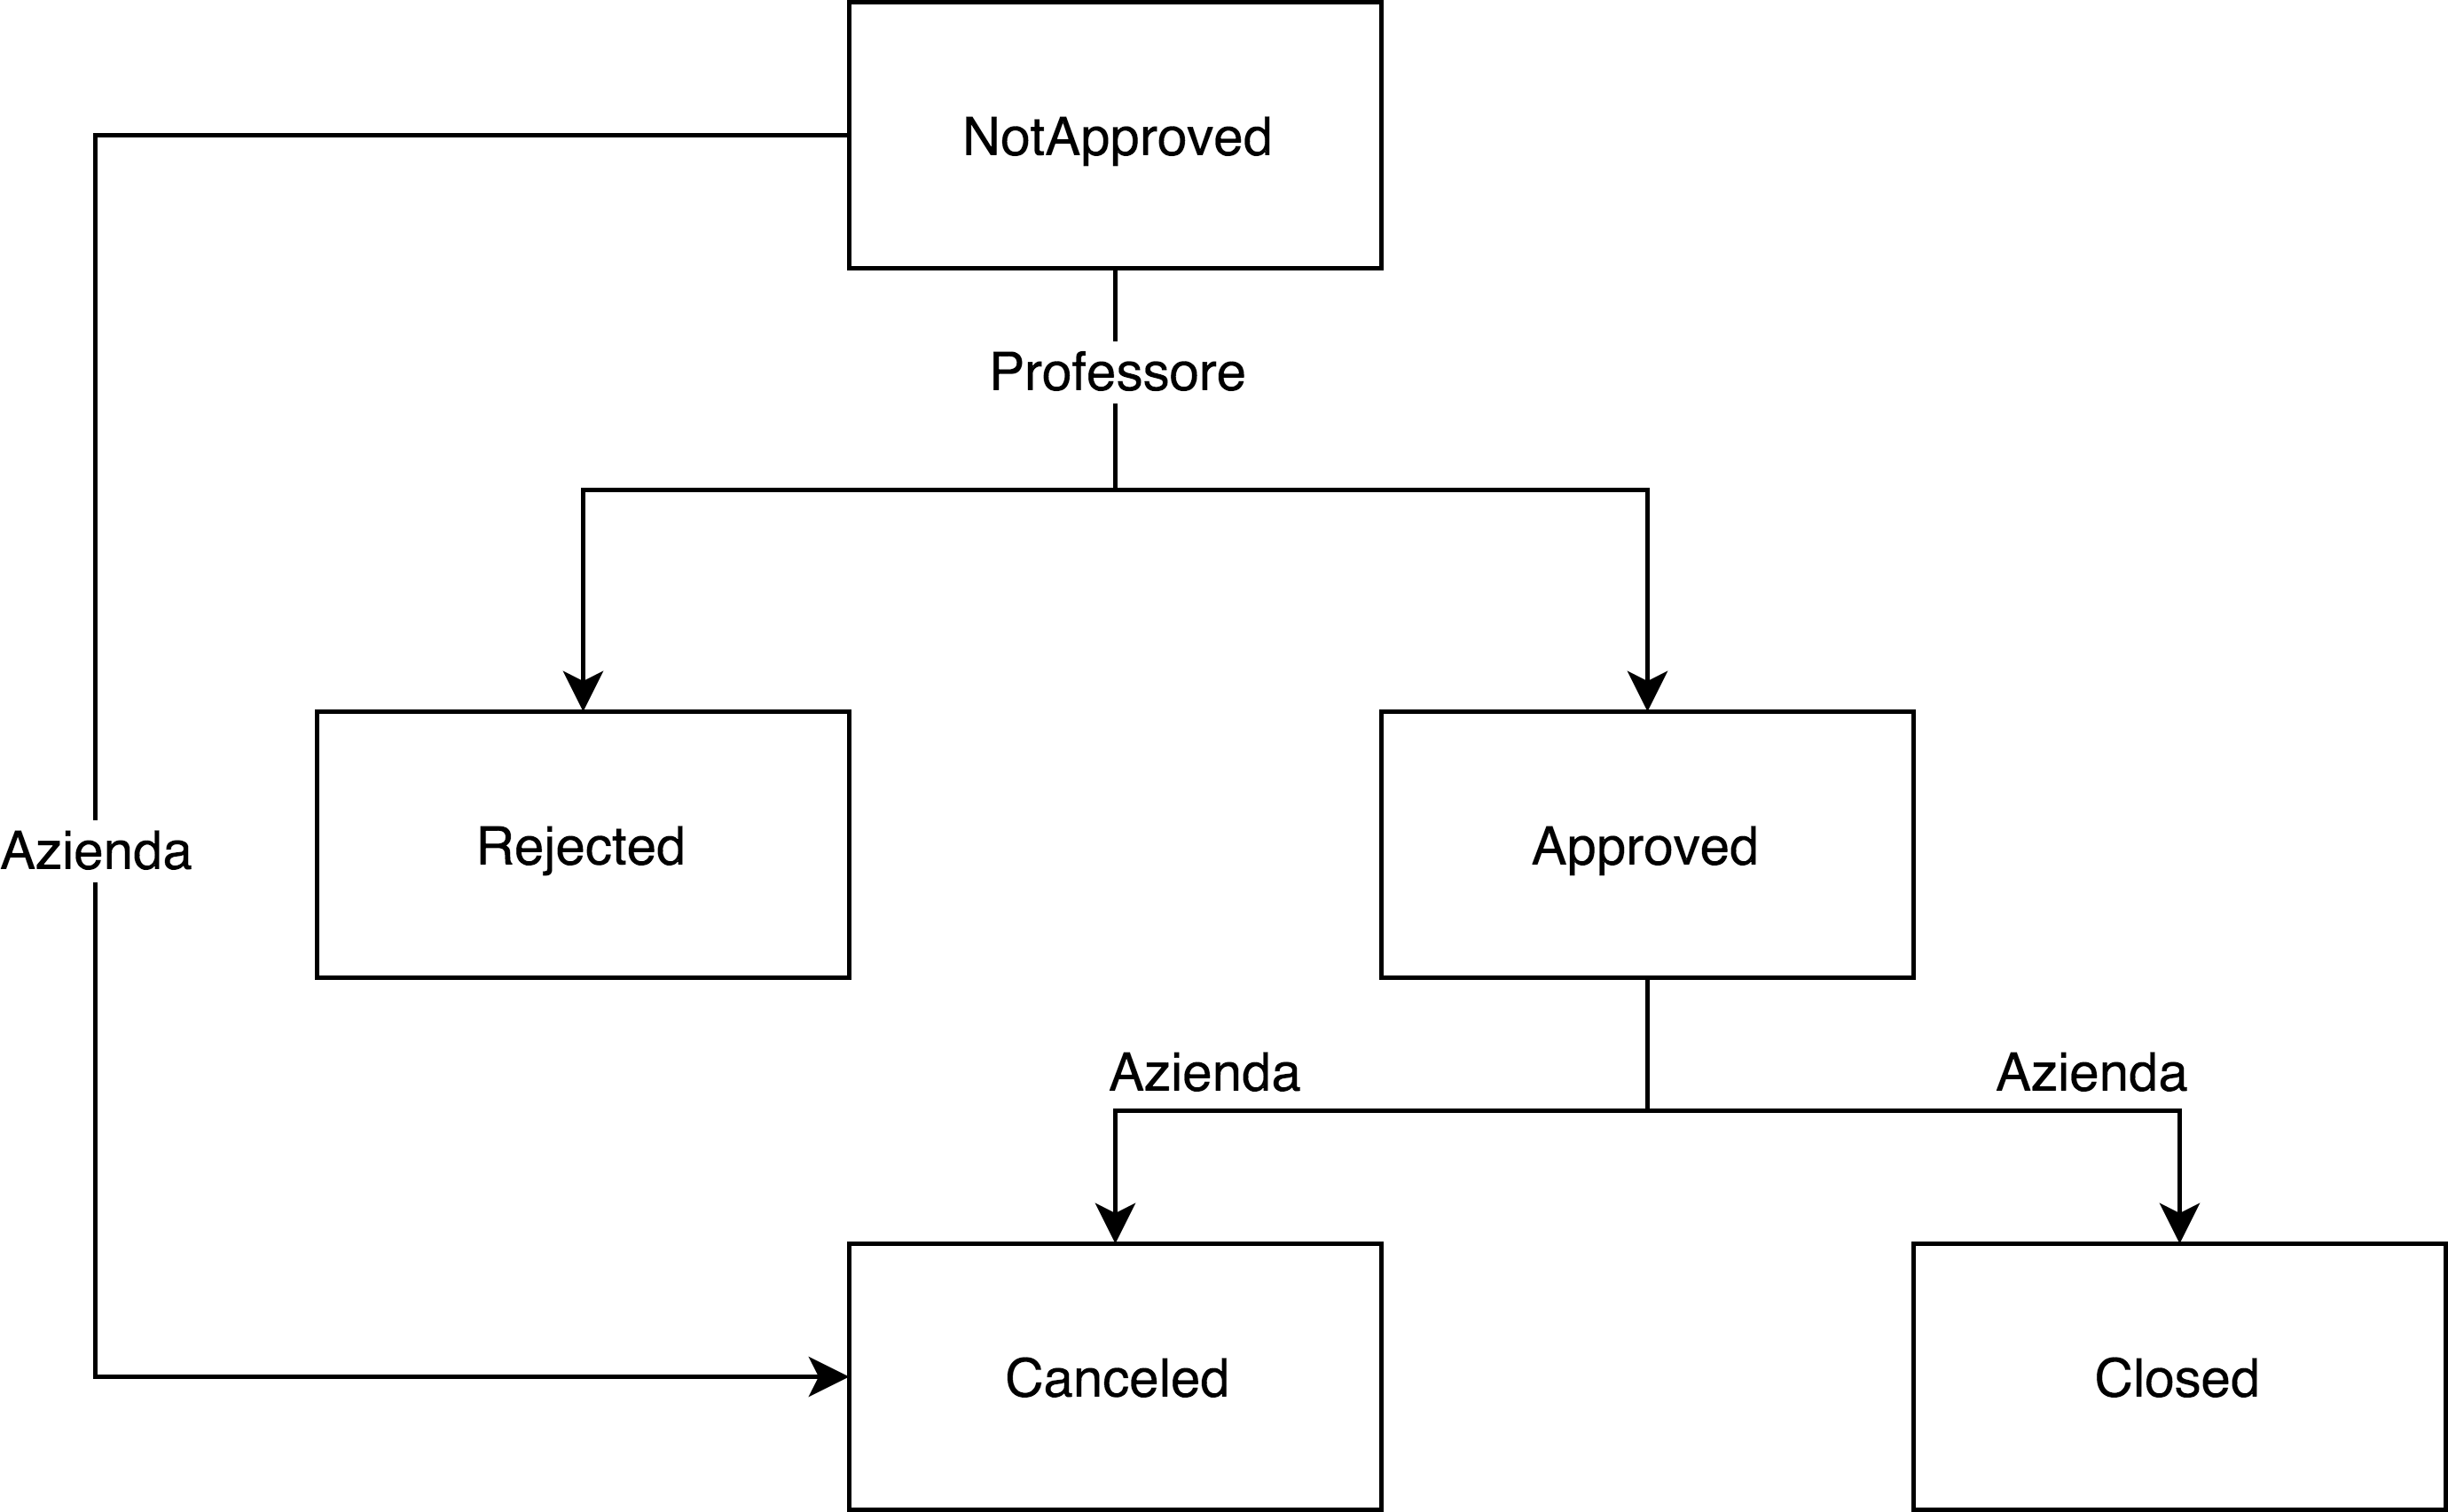
\includegraphics[width=0.5\textwidth]{Chapter4/Figs/internship-state-machine}
		\caption[Macchina a stati di un tirocinio]{Macchina a stati di un tirocinio}
		\label{fig:internship-state-machine}
	\end{figure}
	Nel caso l'utente non abbia il permesso di effettuare la transizione viene ritornato un errore di autorizzazione, mentre se lo stato non è raggiungibile viene ritornato un messaggio di errore che riporta l'errata transizione. In caso di successo viene ritornato il nuovo oggetto aggiornato.
	\item PUT "/status/force": raggiungibile solamente da un utente amministratore, permette di aggiornare lo stato di un tirocinio senza il vincolo della macchina a stati di figura \ref{fig:internship-state-machine}.
	\item GET "/status/:status": ritorna tutti gli stati che l'utente corrente può raggiungere dallo stato passato come parametro.
\end{itemize}

\subsection{InternshipProposalsController}

Questo \textit{controller} gestisce le operazioni sulle candidature ai tirocini. Il suo path è "/proposals".
\subsubsection{Dipendenze}
\begin{itemize}[itemsep=0pt]
	\item \textit{internshipProposalsRepository: InternshipsProposalsRepository}
	\item \textit{companiesRepository: CompaniesRepository}
	\item \textit{internshipsRepository: InternshipsRepository}
\end{itemize}

\subsubsection{Endpoint}
\label{server:internship-proposals-controller}
\begin{table}[H]
	\ttfamily
	\caption{Endpoint \hyperref[server:internship-proposals-controller]{\textit{InternshipProposalsController}}}
	\centering
	\label{table:api:internship-proposals-controller}
	\begin{tabular}{l c c c c}    
		URL  & Metodo & Scope \\ 
		\midrule
		/getByProfessorId/:professorId & GET    \\
		/getByCompanyOwnerId/:companyOnwerId & GET   \\
		/getByStudentId/:studentId & GET   \\
		/availableplaces/:internshipId & GET \\
		/addAttendances & POST & ownInternshipProposalScope \\
		/generateDocs/:internshipProposalId & GET & ownInternshipProposalScope \\
		/status & PUT & ownInternshipProposalScope \\
		/status/force & PUT & adminScope \\
		/status/:status & GET \\
		\bottomrule
	\end{tabular}
\end{table}

Anche in questo caso gli ultimi tre metodi in tabella sono utilizzati per aggiornare lo stato di un tirocinio:
\begin{itemize}
	\item PUT "/status": permette di aggiornare lo stato di una candidatura (es. da "Iniziata" ad "Terminata"). Segue la stessa logica del relativo metodo in \textit{InternshipController}. La definizione della macchina a stati è riportata in figura \ref{fig:internship-proposal-state-machine}.
	\begin{figure}[H] 
		\centering    
		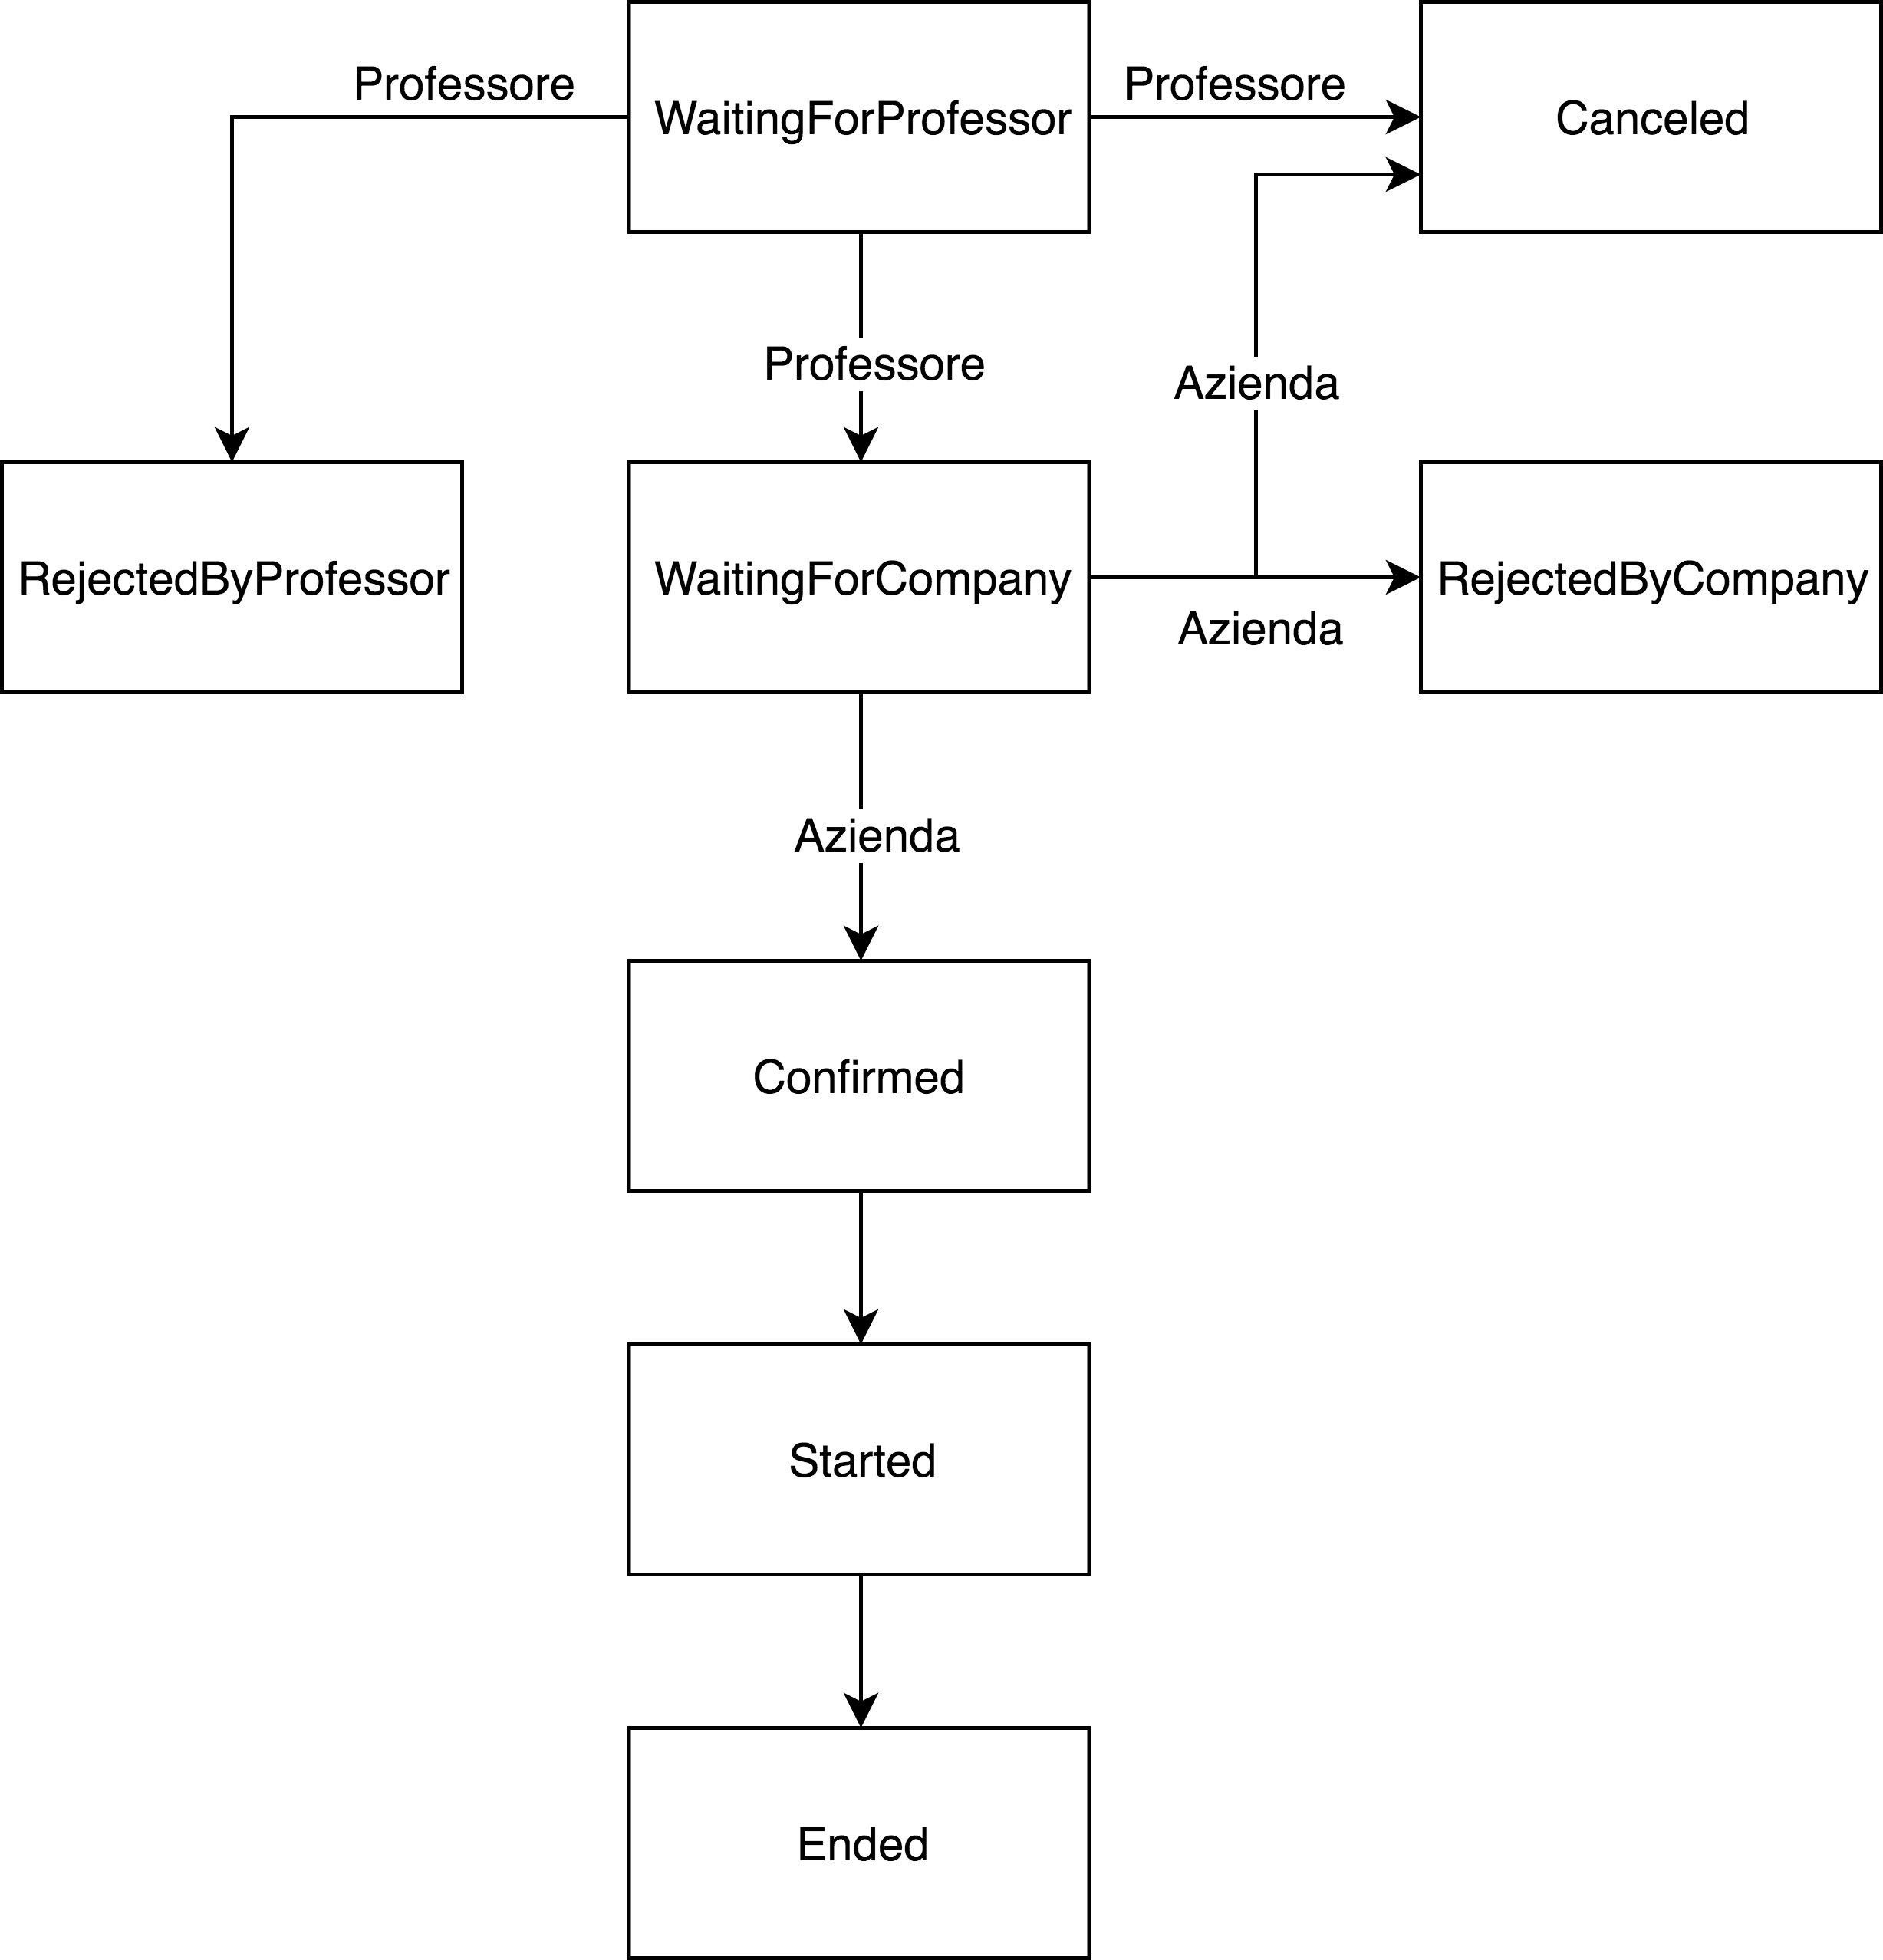
\includegraphics[width=0.4\textwidth]{Chapter4/Figs/internship-proposal-state-machine}
		\caption[Macchina a stati di una proposta di tirocinio (candidatura)]{Macchina a stati di una proposta di tirocinio (candidatura)}
		\label{fig:internship-proposal-state-machine}
	\end{figure}
	\item PUT "/status/force": raggiungibile solamente da un utente amministratore, permette di aggiornare lo stato di un tirocinio senza il vincolo della macchina a stati di 	figura \ref{fig:internship-proposal-state-machine}
	\item GET "/status/:status": ritorna tutti gli stati che l'utente corrente può raggiungere dallo stato passato come parametro.
\end{itemize}

\subsection{RolesController}

Questo \textit{controller} gestisce le operazioni sui ruoli degli utenti. Il suo path è "/roles".
\subsubsection{Dipendenze}
\begin{itemize}[itemsep=0pt]
	\item \textit{rolesRepository: RolesRepository}
\end{itemize}

\subsubsection{Endpoint}

Non ha metodi custom, ma espone solamente le operazioni \acrshort{crud} offerte da \hyperref[server:base-controller]{\textit{BaseController}}.

\subsection{UsersController}

Questo \textit{controller} gestisce le operazioni sugli utenti. Il suo path è "/users". Limita l'utilizzo del metodo di aggiornamento ed eliminazione solamente agli utenti con il ruolo di amministratore, per impedire modifiche non autorizzate agli utenti.
\subsubsection{Dipendenze}
\begin{itemize}[itemsep=0pt]
	\item \textit{usersRepository: UsersRepository}
\end{itemize}

\subsubsection{Endpoint}
\label{server:users-controller}
\begin{table}[H]
	\ttfamily
	\caption{Endpoint \hyperref[server:users-controller]{\textit{UsersController}}}
	\centering
	\label{table:api:users-controller}
	\begin{tabular}{l c c c c}    
		URL  & Metodo & Scope \\ 
		\midrule
		/getByRole/:role & GET    \\
		/own & PUT & ownUserScope   \\
		/professors/lookup & POST   \\
		\bottomrule
	\end{tabular}
\end{table}

\pagebreak
\subsection{CompaniesController}

Questo \textit{controller} gestisce le operazioni sulle aziende. Il suo path è "/companies".

\subsubsection{Dipendenze}
\begin{itemize}[itemsep=0pt]
	\item \textit{companiesRepository: CompaniesRepository}
\end{itemize}

\subsubsection{Endpoint}

\label{server:companies-controller}
\begin{table}[H]
	\ttfamily
	\caption{Endpoint \hyperref[server:companies-controller]{\textit{CompaniesController}}}
	\centering
	\label{table:api:companies-controller}
	\begin{tabular}{l c c}    
		URL  & Metodo & Scope \\ 
		\midrule
		/getByOwnerId/:ownerId & GET    \\
		\bottomrule
	\end{tabular}
\end{table}

\subsection{AuthenticationController}

Questo \textit{controller} gestisce le operazioni di login e registrazione degli utenti. Il suo path è "/auth". Non deriva da \textit{BaseController} in quanto non esporta operazioni sulle entità, ma si preoccupa solamente di verificare l'identità degli utenti e di generare un \textit{token} di accesso. Tutti i suoi metodi sono, per ovvie ragioni, privi di autenticazione e liberamente accessibili.

\subsubsection{Dipendenze}
\begin{itemize}[itemsep=0pt]
	\item \textit{usersRepository: UsersRepository}
	\item \textit{rolesRepository: RolesRepository}
\end{itemize}

\subsubsection{Endpoint}

\label{server:auth-controller}
\begin{table}[H]
	\ttfamily
	\caption{Endpoint \hyperref[server:auth-controller]{\textit{AuthenticationController}}}
	\centering
	\label{table:api:auth-controller}
	\begin{tabular}{l c c}    
		URL  & Metodo & Scope \\ 
		\midrule
		/login & POST &  \\
		/register & POST &  \\
		/google & GET &  \\
		/token/validate & GET  &  \\
		/token/decode & GET  & (solo debug)  \\
		\bottomrule
	\end{tabular}
\end{table}
